\section{Experimental Results}\label{sec:exp}

In this section we describe our experimental setup, and describe and interpret our results for the three different algorithm instances.
The results will compare the naive implementation to the autotuned versions of FWI and FWT both as scalar and vectorized implementations. 

\mypar{Experimental setup}
Due to time constraints, the experiments were run on three different platforms, one per algorithm instance. The respective platform specifications can be seen in Tbl. \ref{tbl:system}. For brevity, the CPU brands are omitted, as all three are Intel CPUs. $\beta$ is a shorthand notation for memory bandwidth in bytes/cycle. 

The source code implementations were compiled with \texttt{clang} version 13.0.1. Vector code was compiled with \texttt{-O3 -ffast-math -march=native}, scalar with \texttt{-O3 -no-loop-unroll -fno-slp-vectorize}. 

Please note that we intentionally added the compiler flags \texttt{-no-loop-unroll -fno-slp-vectorize} and omitted the compiler flags \texttt{-ffast-math -march=native} for scalar code to ensure the compiler did not perform unrolling and vectorization optimizations by itself, thereby confounding our performance measurements. We performed a small search for different compilers and compiler flags to ensure we used the best-possible compiler and flags.

The compiled implementations for APSP and MM were run and measured on input sizes $N \in [432, 4608]$, where the input matrix $C$ consists of randomly generated double-precision floating-point values and has size $N \times N$. For TC, we have $N \in [256, 20992]$ and the input matrix $C$ of size $N \times N$ consists of randomly generated bits. In any case, we collected enough measurements to ensure timing overhead was insignificant and little to no variation could be observed.

In order to obtain measurements for performance and amount of data transferred, we measured the number of cycles and the number of misses in the L3 cache using the PAPI library \cite{terpstra2010papi}. We warm up the cache to ensure proper measurements.

\begin{table}[h]
\centering
\begin{tabular}{ | c | c | c | c | }
 \hline
  & APSP & MM & TC \\ 
 \hline
 CPU & Xeon E3 & Core i7 & Core i7\\
 Base Freq. & 2.8GHz & 1.8GHz & 1.8GHz\\
 $\mu$arch & Skylake & Coffee Lake & Coffee Lake\\
 SIMD & AVX-2 & AVX-2 & AVX-2 \\
 L3 size & 8 MiB & 8 MiB & 12 MiB\\
 $\beta$ [B/cycle] & 6.79 & 7.53 & 7.03\\
 \hline
\end{tabular}
\caption{Specifications of respective platforms}
\label{tbl:system}
\end{table}

\mypar{All-Pairs Shortest Path Results}
%As the naive and unrolled implementations of FW iterate over the input matrix \texttt{C} suboptimally, the computation will likely become memory-bound for larger input sizes. Therefore, we expect our cache-tiled implementations \texttt{FWT} and \texttt{FWT-vectorized} to outperform their non-tiled counterparts \texttt{FWI} and \texttt{FWI-vectorized} for larger input sizes.

Figure \ref{fig:sp-perf} shows the observed performance for the APSP problem. For scalar code, the tiled FWT
code achieves 3.3x speedup relative to the naive implementation and 110\% of the theoretical peak scalar performance
as there seems to be a bug in the autotuner which leads it to generate vectorized code for the scalar implementations.
For vector code, the tiled FWT significantly outperforms the non-tiled counterpart and achieves 9.5x
speedup relative to the naive implementation and 78\% of the theoretical peak SIMD performance.

Interestingly, the tiled, non-vectorized code outperforms the non-tiled, vectorized code for larger
input sizes. In fact, we see that the performance of the non-tiled, vectorized implementation
converges to that of the non-tiled, non-vectorized implementation. We can explain this result using
the roofline model \cite{williams2009roofline}. Figure \ref{fig:sp-roof} shows the roofline plot for
the APSP problem. Smaller input sizes are show with smaller dots and larger input sizes with larger dots.
The plot shows that non-tiled implementations quickly become memory-bound while tiled implementations
remain compute-bound.

Around $N = 2880$ we see a pronounced drop in performance for FWT-SIMD and less pronounced for the scalar FWT.
There are a few possible explanations for this drop. One possibility is that the hill-climbing during the autotuning
settled on a suboptimal local-maximum, which is possible due to the severe non-convexity of the parameter space.
Another possibility is that the autotuner is limited in its choice of legal tile sizes due to the divisibility of
the input size. The fact that 2880 is highly divisible (in fact even more divisible than the adjacent input sizes) speaks
against the latter option. But the observation that the vectorized implementation is much more affected speaks for the
latter possibility, as vectorization reduces the set of legal tile sizes.

All in all, we can see that the autotuner is able to successfully apply effective optimizations to the Floyd-Warshall
algorithm.

\begin{figure}[h]
    \centering
    \includegraphics[width=0.47\textwidth, keepaspectratio=true]{sp-optimizations-large_perf.eps}
    \caption{Performance comparison of FW implementations for APSP.}
    \label{fig:sp-perf}
\end{figure}
\begin{figure}[h]
    \centering
    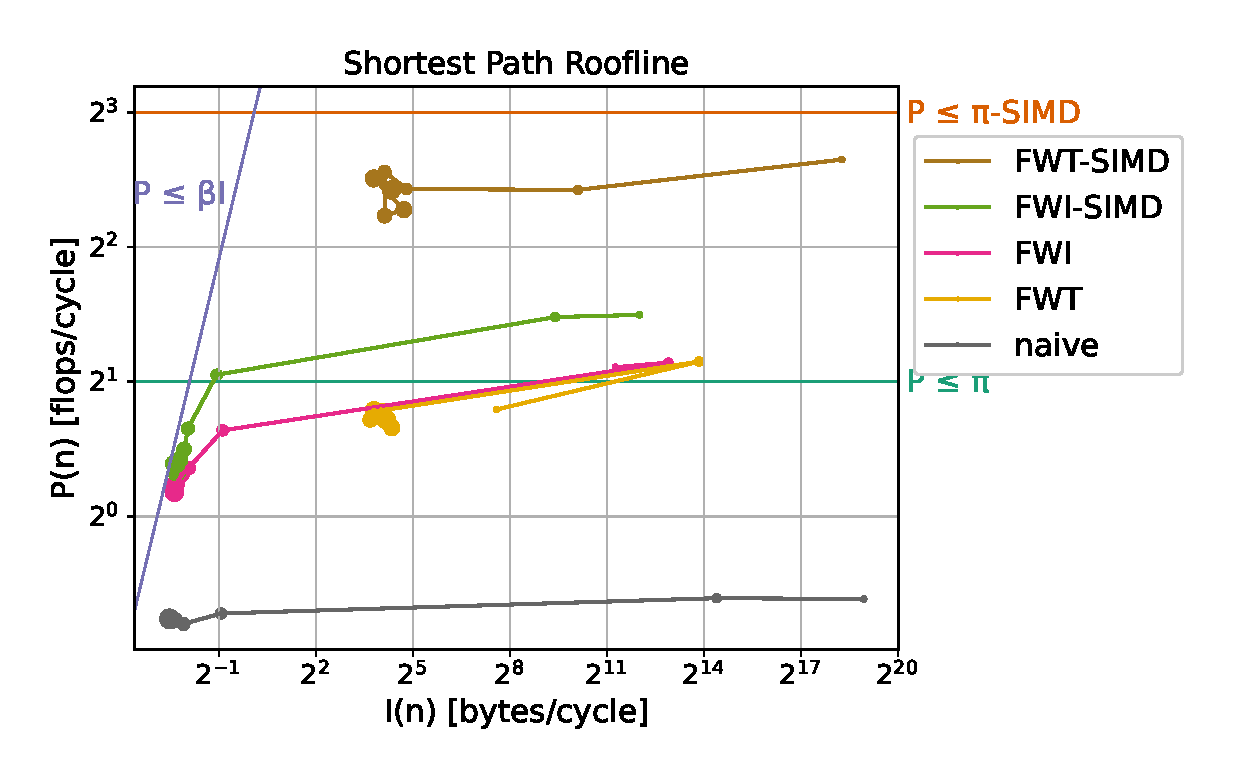
\includegraphics[width=0.47\textwidth, keepaspectratio=true]{sp-optimizations-large_roof.eps}
    \caption{Roofline plot of FW implementations for APSP.}
    \label{fig:sp-roof}
\end{figure}


\mypar{Max-Min Results}
As the structure of the computation, the instruction latency and throughput, as well as the data structure and representation
is identical to that of the APSP instance, we expect our optimizations to reach similar performance values for the MM instance.

Figure \ref{fig:mm-perf} shows the performance of the MM implementations. For scalar code, the tiled FWT code achieves
2.2x speedup relative to the naive implementation and 103\% of peak scalar performance because of the bug in the autotuner.
For vector code, the tiled FWT significantly outperforms the non-tiled counterpart and achieves 6.1x speedup relative to
the naive implementation and 72\% of the theoretical peak SIMD performance. 

Similarly to the APSP instance, the performance for both tiled implementations shows a dropoff at $N = 2304$. This is interesting
as it would be odd for the autotuner to manifest the same quirk to find a suboptimal local maximum for the same region of
input sizes. It is not impossible, however, as the performance for $N = 2880$ shows improvement which it did not do
for the APSP instance.

Looking at the roofline plot in figure \ref{fig:mm-roof} we find the same characteristic for the MM instance that only tiled
implementations manage to stay computationally bounded. This is an example of one autotuner being able to effectively
apply the same optimizations to two different algorithms.
\begin{figure}[h]
    \centering
    \includegraphics[width=0.47\textwidth, keepaspectratio=true]{mm-optimizations-large_perf.eps}
    \caption{Performance comparison of FW implementations for MM.}
    \label{fig:mm-perf}
\end{figure}
\begin{figure}[h]
    \centering
    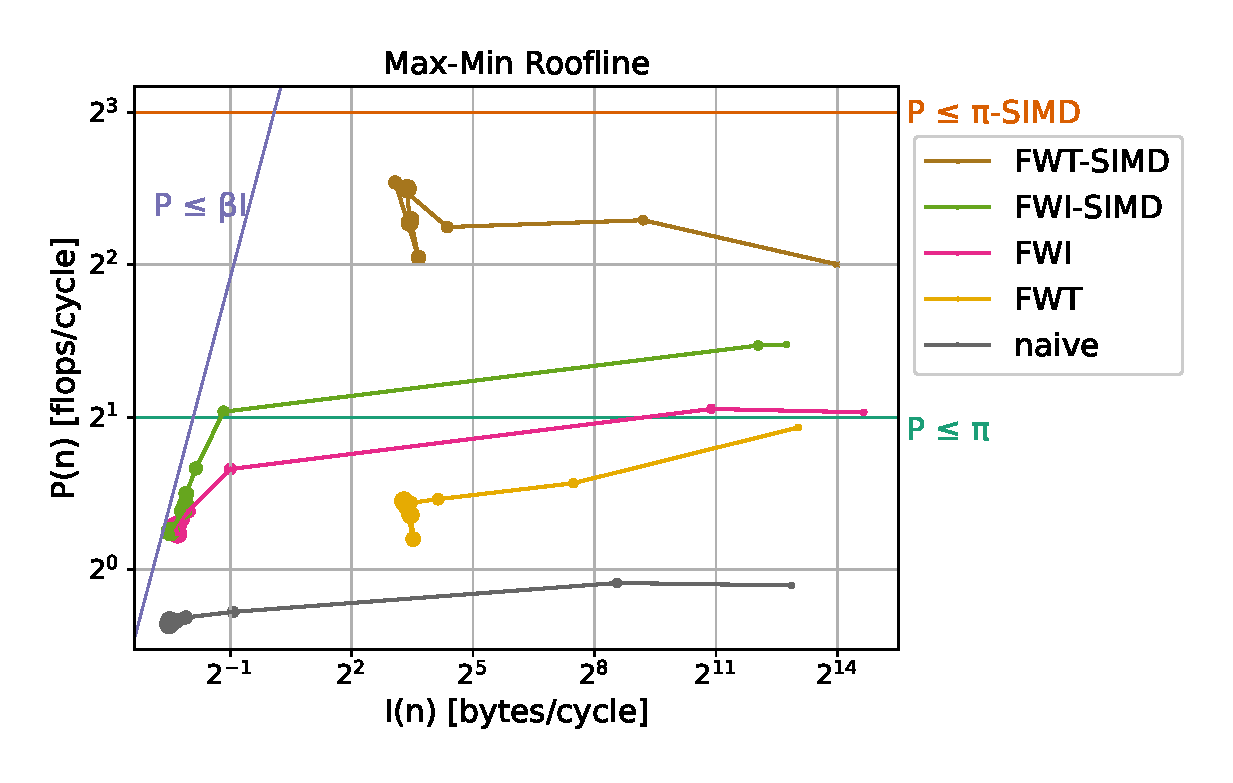
\includegraphics[width=0.47\textwidth, keepaspectratio=true]{mm-optimizations-large_roof.eps}
    \caption{Roofline plot comparing implementations for Max-Min on an Intel Core i7 (Coffee Lake microarchitecture).}
    \label{fig:mm-roof}
\end{figure}

\mypar{Transitive Closure Results}
The TC instance, while following the same algorithmic and data structure has a different data representation and instruction
latency and throughput. As a result, it is not a given that the optimizations translate to this instance.

Figure \ref{fig:tc-perf} shows the performance plot for the TC instance. The scalar FWT implementation achieves 65\% of the
theoretical scalar peak performance. However, due to finding and fixing a bug too close to the deadline, we were not able to run the measurements
for all input sizes as running the autotuner takes considerable amount of time, especially for the large input sizes. The
vectorized FWT implementation achieves a 33.3x speedup compared with the naive implementation and 65\% of the theoretical
SIMD peak performance.

Note that the vectorized tiled implementation exhibits large, intermittent dropoffs in performance. In this case we know that this
is caused by a constriction of the parameter space for certain input sizes leading to the optimal tiling factors not being available
for selection by the autotuner. The lack of legal optimal tiling factors is due to the bit-packing, which packs 256 bits into a
single vector register. Therefore, the number of available factors and therefore tiling factors diminishes considerably.

Looking at the roofline plot in figure \ref{fig:tc-roof} we see that, while both vectorized implementations initially display 
similar performance characteristics, the fact that,  like for the other instances, only the tiled implementations remain
compute-bound, the tiled implementation performs better for large input sizes.

This shows that the autotuner was still able to successfully apply the same optimizations and achieve a similar result
even for different data representations and different instruction latencies and throughputs. However, the TC instance
also shows limits to the generality of our autotuner. While the vectorized FWT remained compute bound, its performance
was severely decreased as a consequence of the different data representation with the bit-packed vectors.
However, the different instruction latencies and throughputs do not impact the performance, as an autotuner
finds the optimal values empirically.

\begin{figure}[h]
    \centering
    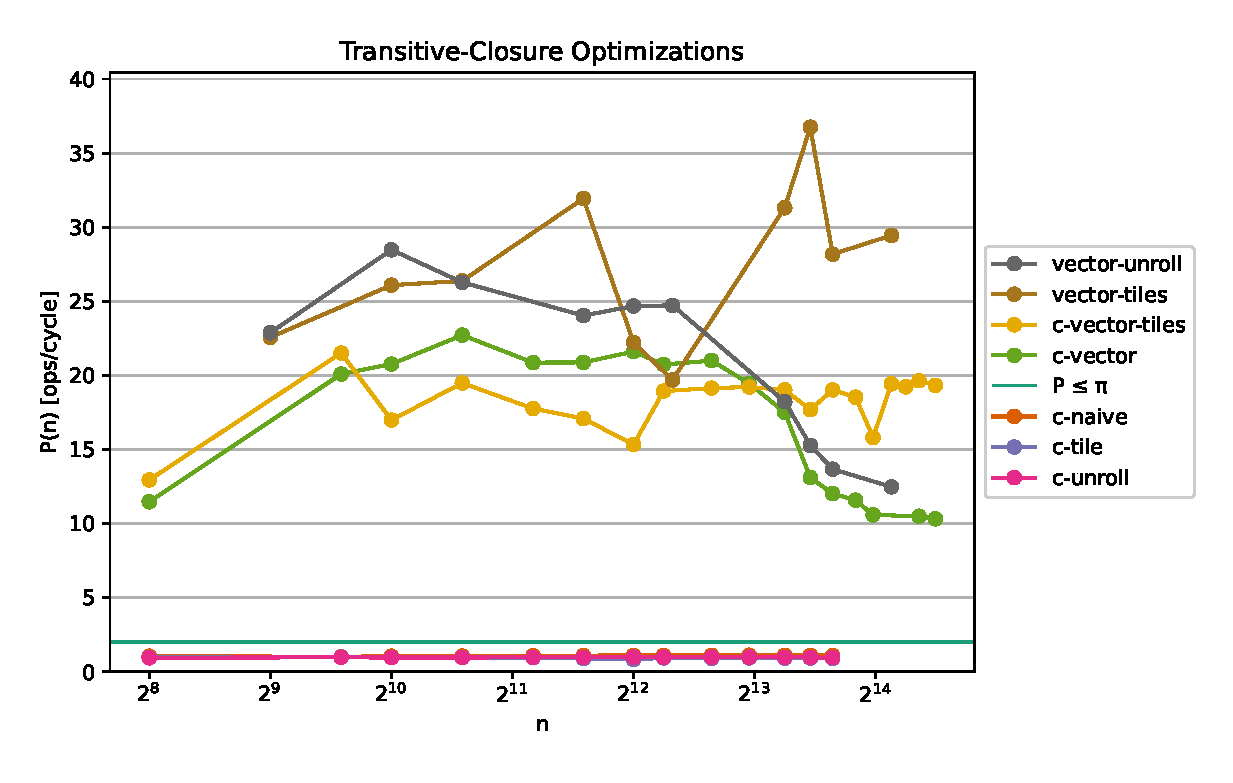
\includegraphics[width=0.47\textwidth, keepaspectratio=true]{tc-optimizations-large_perf.eps}
    \caption{Performance comparison of FW implementations for TC.}
    \label{fig:tc-perf}
\end{figure}
\begin{figure}[h]
    \centering
    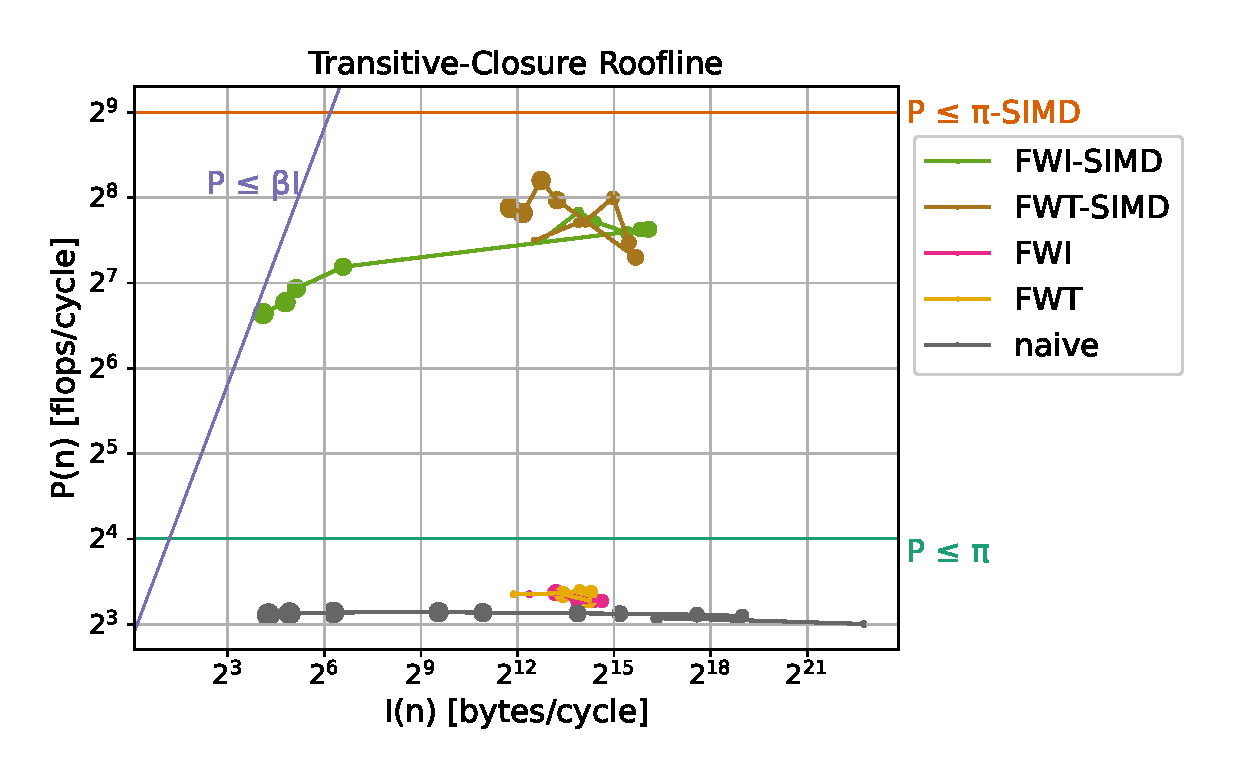
\includegraphics[width=0.47\textwidth, keepaspectratio=true]{tc-optimizations-large_roof.eps}
    \caption{Roofline plot comparing implementations for Transitive Closure on an Intel Core i7 (Coffee Lake microarchitecture).}
    \label{fig:tc-roof}
\end{figure}